\section{Background}

\subsection{GPS Positioning}
\begin{figure}
    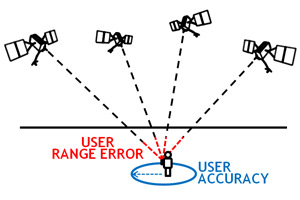
\includegraphics[scale=0.5]{figures/gps-how.jpg}
    \caption{From \cite{gpsGov}: GPS Technology Overview}
\label{fig:gps:how}
\end{figure}


GPS Positioning technology makes use of satelites in known orbits around the earth, broadcasting the current time. By consulting the orbits and the time taken for a signal to arrive from a number of satelites, GPS recievers can determine their own location on Earth, as shown in \figref{fig:gps:how}.

\begin{figure}
    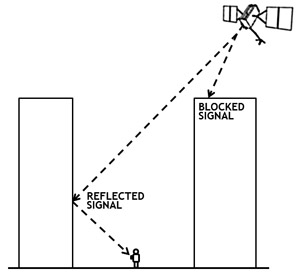
\includegraphics[scale=0.5]{figures/gps-reflect.jpg}
    \caption{From \cite{gpsGov}: GPS sources of error - reflected signals.}
\label{fig:gps:reflect}
\end{figure}


However, GPS cannot produce perfectly precise locations. Error is introduced by a variety of factors: Orbital information can be out-of-date or subtly incorrect, or too few satelites may be within reach. \figref{fig:gps:reflect} shows a more dramatic problem, in which the signal recieved is bounced off a nearby object before being received.

\subsection{Path Refinement}

GPS positions inherently include measurement error, as mentioned above, but naive attempts to interpolate between positions can cause dramatically more error if done poorly. Lonergan \textit{et al.} demonstrated that point-connecting strategies such as linear or quadratic interpolation have error that scales linearly with the time between GPS positions when tracking wild animals~\cite{lonergan09}.

Different strategies can be applied to refine positions within a \textit{path}, depending on the goal. If attempting to determine the length of the path, map-matching techniques allow a path to be overlaid on a known (and presumably accurate) network. Conversely, if the goal is to extract a more accurate path, sensor readings can be combined with additional information and rules.

Path refinement is extremely difficult to evaluate, as the underlying premise is that the sensor data provided is inaccurate. As a result, evaluation of such techniques tends to focus around path \textit{recoverability}, in which the sensor data is randomly permuted across trials, and the similarity of the refined paths is compared.
